%=============================================================================
% DATA AND PROTOCOL
%=============================================================================
\section{Data and Evaluation Protocol}
\label{sec:setup}

\subsection{Data}
\cA{We use the processed national surveillance array of Weng
et al.~\cite{weng2024graph}: 459 weekly observations for Sri Lanka's 25
districts (2013--2022), weekly reported cases as the target, ten lag-shifted
climate covariates, and a district graph of 141 directed edges with self-loops.
The target is heavy-tailed (median 13, maximum 2631, 9.7\% zeros, skewness 8.6),
so we model $\log(1+y)$. The dominant statistical fact is temporal, not spatial:
cases at $t-1$ explain $r^2=0.85$ of cases at $t$, while the best single
covariate explains $0.02$. Every number below should be read against that.}

\subsection{Protocol}
\cB{We use rolling-origin (expanding-window) cross-validation with three
chronological origins ($0.55, 0.70, 0.85$ of the series) and three seeds, a
$W=3$ week input window and an $H=3$ week horizon. Normalisation statistics are
computed from training weeks only and recomputed per fold; no shuffling occurs at
any point. Model selection uses a genuine validation split of the final 30
training weeks, and we report \emph{pooled} RMSE over held-out windows.}

\cB{Three of those choices are corrections to the reference protocol rather than
preferences, and \S\ref{sec:repro} quantifies each.}

\subsection{An evaluation artifact, and dual scoring}
\label{sec:artifact}

\cC{Exploratory analysis identified week~395 as a $19\times$ spike in reported
cases occurring simultaneously in 18 of 25 districts. A simultaneous
multi-district jump of that magnitude is an administrative reporting backlog, not
an epidemiological event.}

\cC{Under our protocol it falls in the \emph{test} split of the origin-0.85 fold
and in no training split at all. Six of that fold's 68 windows touch it, and they
carry approximately 90\% of its squared error (Fig.~\ref{fig:artifact}).
Persistence scores RMSE 68.62 over all 68 windows, 219.07 over the six, and 22.80
over the remaining 62.}

\begin{figure}[t]
  \centering
  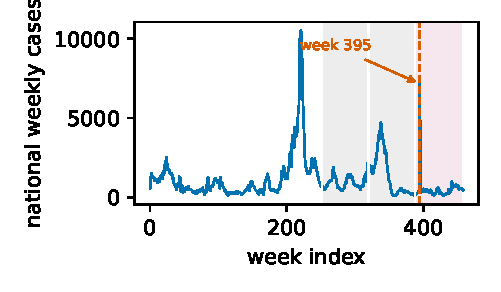
\includegraphics[width=\linewidth]{figures/fig_artifact}
  \caption{The national series, with the three test splits shaded. The week-395
  backlog lands in the last one. On that fold persistence scores RMSE 68.62 over
  all 68 windows, 219.07 over the six touching week~395, and 22.80 over the
  remaining 62.}
  \label{fig:artifact}
\end{figure}

\cD{This has two consequences that any benchmark on this dataset inherits. First,
the fold ordering inverts: measured over all windows, origin~0.85 is by far the
hardest fold (68.62 against 26.88 and 38.89); measured artifact-free it is the
\emph{easiest} (22.80). A claim about ``the hard fold'' is therefore meaningless
without stating which scoring it came from. Second, because that fold dominates
the pooled average, the persistence floor itself moves---from RMSE 44.80 to
\textbf{29.52}---and so does every model's apparent margin against it.}

\cD{We therefore score every arm twice: over all test windows, and over the
artifact-free subset. Crucially the \emph{baseline is split the same way}. Scoring
a model artifact-free against a floor computed over all windows compares two
different test sets. We do not drop the windows silently, because doing so
flatters every arm equally and conceals that a fold's difficulty was one week of
bad data.}
